% ===========================================================================
% v3 §5 — THE STEERING LOOP: LEARNING WITHOUT GRADIENTS (~2 pp; F4, F7, T2)
% Draft r1 (2026-09-03), claims block with §6 and §10 (decision 20). Replaces v2 §4 "Learning Without
% Gradients" (v2:505-609): first two paragraphs and the two episodes kept in substance; the register and
% the enforcement hierarchy (from v2's "operating skeleton") moved here; the id-collision worked example added;
% divergence learning kept; K/freeze stated as the exit rule with "not yet exercised".
% Counts (census 2026-09-03): 43 heading-form numbered lessons in the five step skills that carry them
% (L 31 present of ids to 34, TM 5, D 5, G 2, T 11 — dev/build_learning_curve.py census); register 49 NR
% rows: 20 DEPLOYED, 21 PROPOSED, 3 PARTIAL, 5 closed/practice/fix-applied; 9 rows with a keep: clause.
% Figure F4 = figures/fig_F4_steering_loop (gated); F7 = figures/fig_F7_learning_curve (dev/build_learning_curve.py).
% Decisions 18/19: describe what runs; no claims. \cite keys are v2's (in agentic_grb.bib).
% ===========================================================================
\providecommand{\rc}[1]{\parbox[t]{10.2cm}{\raggedright #1}}   % register-table cell; move to the preamble at splice
\section{The Steering Loop: Learning Without Gradients} \label{sec:learning}

Contemporary AI agents are improved in five ways: pretraining on large
corpora; supervised fine-tuning on demonstration trajectories; preference
optimization against human or model judgments; reinforcement learning on
\emph{verifiable} rewards, where a trajectory is reinforced only if its
outcome can be checked mechanically; and \emph{harness-side learning}, in
which the model's weights are never touched and the surrounding harness,
its instructions, procedures, and memory, accumulates capability instead
\citep{2025Natur.645..633G,2023arXiv230516291W,2023arXiv230311366S}. Our
campaign is training of the fifth kind carrying the fourth kind's essential
ingredient. The weights of every model we use are frozen; the artifact that
learns is the skill library; and the unit of learning is constrained to be
verifiable: a lesson enters the library only as a claim with provenance
(which burst, which date, which evidence) together with an executable test
that fails if the lesson is ever violated again. The suite runs against the
current analysis products; where a table predates a fix, the failure is
registered in a known-stale ledger with its clearing condition rather than
silenced. Debt is visible, never normalized.

Figure~\ref{fig:steering} draws the loop that produces the lessons. An
\emph{incident} is a defect caught by anyone: a verifier, a test, the
external auditor, or the human at a gate. A \emph{prior-art reader} asks
first whether the project has already proven the point, because
re-deriving a known result is the campaign's most expensive habit. The
\emph{distiller}, in the same session that saw the incident, drives the
root cause to the primitive and chooses the strongest enforcement layer
that can hold the countermeasure: code over hook over artifact over agent
over prose. A rule that can be a test becomes a test; a rule that can only
be a sentence in a skill file is written as one and marked as the weakest
layer. The countermeasure is then recorded twice: as a numbered lesson in
the step's skill file, and as a row of the requirements register that
names the incident that bore it, the layer chosen, and whether the guard is
deployed or proposed. Nine rows so far carry a \emph{keep} condition, the
observable that would show the guard no longer holds. The loop closes on
the next burst, which runs a better pipeline.

\begin{figure*}[t]
\centering
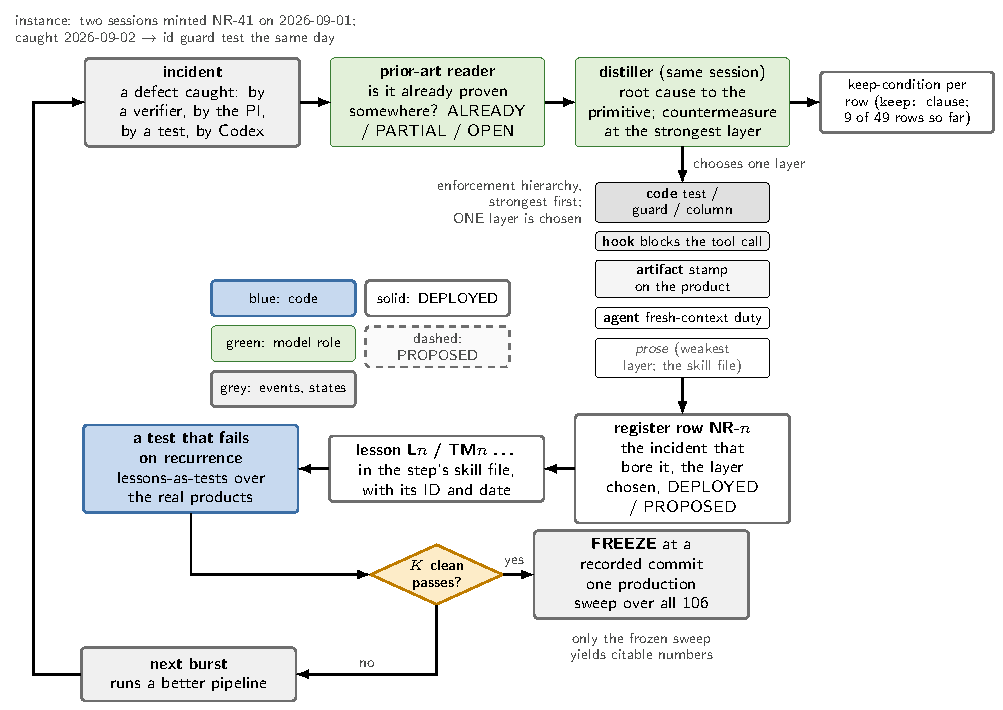
\includegraphics[width=0.95\textwidth]{figures/fig_F4_steering_loop.pdf}
\caption{The steering loop. An incident, caught by a verifier, a test, the
external auditor, or the human, passes a prior-art reader and a distiller
(green: model roles) that place the countermeasure at the strongest layer
of the enforcement ladder (grey rungs, graded by strength), then record it
as a register row and a numbered lesson (white: documents) with a test that
fails on recurrence (blue: code). The amber diamond is the human's decision
to declare convergence after $K$ clean passes; the freeze and the single
production sweep follow. Neither has yet occurred: $K$ is not set and no
clean pass has been recorded.}
\label{fig:steering}
\end{figure*}

This training style has properties that gradient methods cannot offer at
our scale, and one property they share. It is data-efficient: the five
step skills that carry lessons hold forty-three numbered lessons\prov,
twenty-seven of them attributed to the nine bursts walked so far and the
rest to the campaign batches between walkthroughs. It is auditable: the learned policy is plain
text, and every rule cites the burst that paid for it. It transfers across
model families: the same library is executed by different vendors' agents,
which is the basis of the multi-system comparison of \S\ref{sec:design}.
It survives model upgrades. And, the shared property, it exhibits a
learning curve (Fig.~\ref{fig:curve}), whose flattening is the campaign's
stopping criterion: when $K$ consecutive bursts produce no new lesson, the
library is declared converged, the pipeline is frozen at a recorded commit,
and the whole sample is re-analysed once by the frozen system. Only that
sweep produces citable numbers.

\begin{figure}[t]
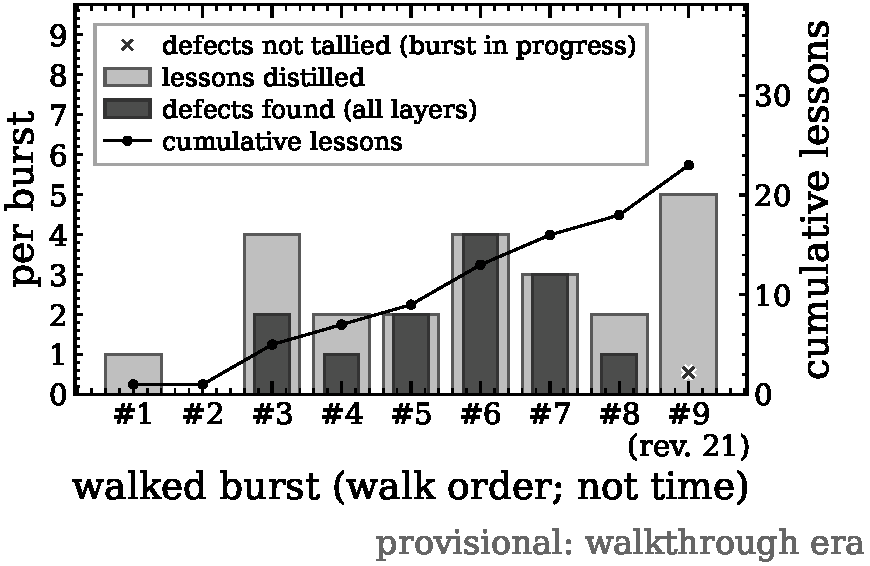
\includegraphics[width=\columnwidth]{figures/fig_F7_learning_curve.pdf}
\caption{The campaign learning curve\prov: lessons distilled per walked
burst (bars), engine defects found (dark bars), and the cumulative lesson
count (line), from the campaign ledger for the first eight walked bursts
and from the dated lesson entries for the walkthrough burst still in
progress. The curve is visibly unconverged; its flattening, not a preset
burst count, terminates the training phase.}
\label{fig:curve}
\end{figure}

\subsection{The register} \label{sec:register}

The register is the campaign's institutional memory: forty-nine numbered
rows\prov, one per needed guard or agent, each carrying the incident that
revealed the need, the layer chosen, and the status. Table~\ref{tab:register}
summarises it and shows eight rows in full. Twenty rows are deployed,
twenty-one are proposed, three are partial (the sensor side built, the
producer side not), and five are closed or recorded as practice. The
dispatcher reads the register at every task intake, so a missing guard is a
stated liability rather than a silent gap, and the register's own rule
applies to itself: a row is minted in the session that saw the incident,
and a proposed guard is listed as proposed until code or a file exists.

\begin{deluxetable*}{lll}   % aastex deluxetable rejects p{} columns; wrapped cells via \rc
\tabletypesize{\footnotesize}
\tablecaption{The requirements register: summary and eight rows in full (census 2026-09-03).\label{tab:register}}
\tablehead{\colhead{row} & \colhead{purpose (the incident that bore it)} & \colhead{status}}
\startdata
\multicolumn{3}{l}{\textit{summary: 49 rows; 20 deployed, 21 proposed, 3 partial, 5 closed or practice; 9 with a keep condition}} \\
NR-1 & \rc{band-validity guard: containment and railed-fraction checks before any spectral band ships (the montage that contradicted its own engine table)} & deployed, code \\
NR-19 & \rc{invalidation cascade: an amended approval clears downstream markers and demotes later approvals mechanically} & deployed, code \\
NR-22 & \rc{skip-by-existence is not skip-by-currency: a marker certifies that a product exists, not which inputs built it} & proposed \\
NR-24 & \rc{report-conformance gate: an assembled deliverable verified against the report contract, including hash equality of report, figures, and table} & proposed \\
NR-30 & \rc{dispatch-hook coverage: the hook that requires a dispatch plan covers one of five launch paths} & proposed \\
NR-44 & \rc{margins-only reporting: information-criterion differences, never absolute values, on this engine} & deployed, code \\
NR-47 & \rc{two-hat separation: the external auditor is never supervisor and blind referee on the same product version} & deployed, protocol and machinery \\
NR-48 & \rc{derived columns recomputed on cell replacement: a promoted table's stored winner must equal the validity-gated argmin over all model columns} & partial (sensor deployed, promotion path proposed) \\
\enddata
\end{deluxetable*}

\subsection{Three episodes} \label{sec:episodes}

Three episodes show what the loop learns and how. The first is a defect we
designate L27. The engine's validity gates flagged a fitted parameter as
railed when it sat within a fixed \emph{linear} margin of its bound. For
energy-like parameters bounded across three decades, that linear margin is
an absolute dead zone of tens of keV above the lower bound, and every burst
analysed in the campaign's first seven walkthroughs had a peak energy far
above it. The eighth burst was soft ($\Ep\sim50$--140~keV\prov), and the
gate silently disqualified every one-break continuum in most of its time
bins, delivering the blocks to thermal-composite models by forfeit.
Uncorrected, the census would have manufactured a population-level
correlation between spectral softness and thermal components, a selection
bias in the costume of physics. The repair (margins computed in the
parameter's natural geometry), its unit test, and the burst's refit
happened within the same session; the pre/post contrast, most blocks
``preferring'' extra structure before and none after\prov, is the measured
size of the bias the lesson prevents. The episode is also an argument about
curricula: the defect was invisible until the sample's serial ordering
happened to deliver a soft burst, so regime coverage, not burst count, is
what a training sample must supply.

The second episode is a cross-validation. Our temporal chain carried a
known, ledgered defect: a spectral-lag sign convention inverted with respect
to the field's standard. The eighth burst has a published lag of
$+7.08\pm0.45$~s in the conventional sign \citep{2018ApJ...865..153L}; our
chain returned $-5.99$~s\prov. Same burst, same physical direction, opposite
sign: the ledgered inversion was confirmed against external ground truth in
the course of ordinary operations, and the lesson (state the convention
with every quoted lag; validate the sign against a burst with a published
direction) was distilled with the defect still unfixed at source. The
library records what is \emph{known}, including known-broken.

The third episode is about the loop itself. On 2026 September~1 two
sessions working the same repository each minted a register row numbered
NR-41, for two different guards. The collision was caught the next day when
the building session inventoried the register, and it was closed the same
day at the strongest feasible layer: one row was renumbered, and a test
that fails on any duplicate identifier entered the suite. The same test now
guards the lesson prefixes of every skill file. The incident cost nothing
scientifically and everything procedurally: a register that can hold two
truths under one number cannot be the campaign's memory, and the fix is a
sentence nobody has to remember.

\subsection{Divergence learning} \label{sec:divergence}

Failures are not the only teacher. Where the human's decision and the
agent's proposal diverge and both are defensible, the divergence itself is
the signal, and it is processed under a fixed protocol: detect it; elicit
the human's reason \emph{in their own words} (a guessed rationale is
forbidden; if the human cannot recall, the record says so); validate the
stated reason against the primitives; generalise it only through a
measured census over the sample, never from the single case; and enter it
in a divergence ledger. The founding case is a detector-selection
divergence: the written geometric rule and two independent agent passes
selected seven detectors\prov; the human had selected four\prov. The human's
recollected reason, keep the detectors that triggered the instrument plus
the companion detector on the same spacecraft side, validated exactly
against the mission's trigger record, and reproduces the detector choice of
every published analysis of that burst we harvested. A census of the full
sample\prov{} then measured how much of expert practice that candidate rule
explains: about eighty percent\prov, with the remainder requiring judgment
the written rule does not capture. The written selection rule therefore
stands unamended, and the divergence is recorded as a measurement of
practice, not promoted to a decision rule. The same census exposed a
contract gap: none of the 105 human selection records\prov{} carried a
contemporaneous reason; the single filled record is a retroactive
reconstruction and is stamped as such. Rationale capture at decision time
is now a registered requirement, while the historical blanks stay blank. A
reconstructed reason is never a contemporaneous record. The ledger gives
the paper's closing question its instrument: the convergence rate, how
often the agent's proposal already matches the human's decision, is the
measurable readiness criterion for ever moving a human gate to an
independent approver.
